\level{2}{Chuck}

	\begin{figure}[H]\centering
        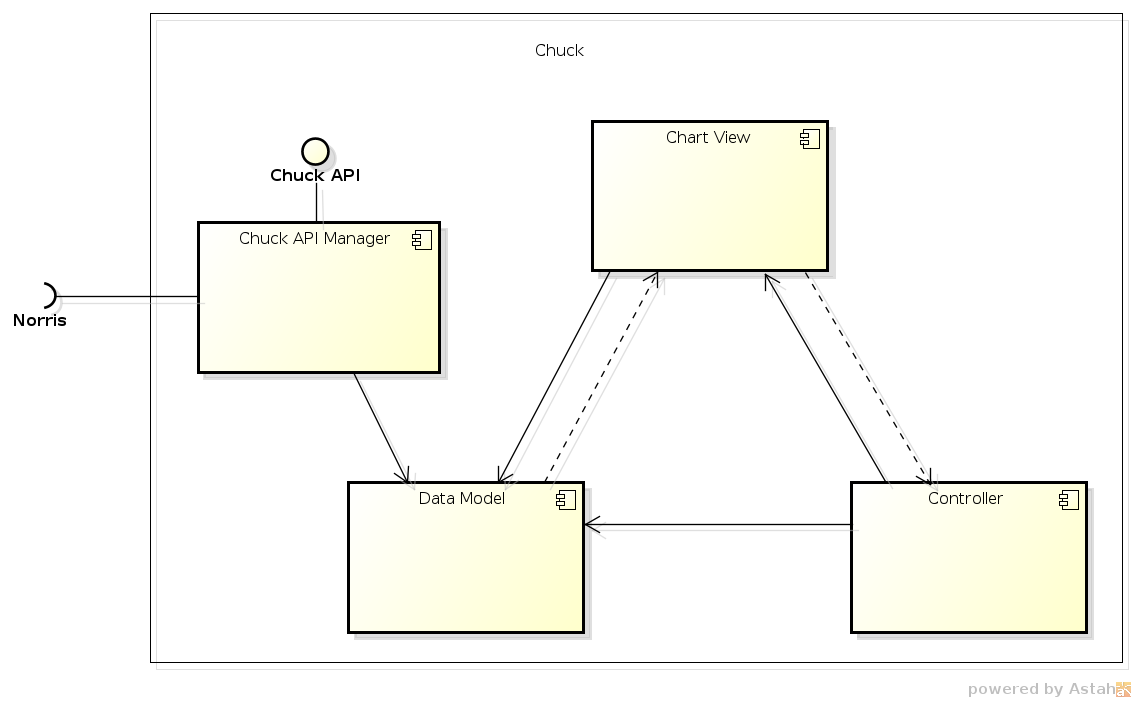
\includegraphics[width=\textwidth]{SpecificaTecnica/Pics/componentiChuck}
        \caption{Diagramma delle componenti di Chuck}
    \end{figure}

    \level{3}{Descrizione dei componenti di Chuck}
    	\level{4}{Chuck API Manager}
    		La componente Chuck Api Manager si occupa di implementare le funzionalità offerte dalle API di Chuck allo sviluppatore client. Queste funzionalità sono:
    		\begin{itemize}
						\item inserimento di nuovi grafici in un sito web;
						\item scelta del tag HTML in cui inserire un grafico;
						\item modifica di alcune impostazioni dei grafici;
						\item login;
						\item logout.
			\end{itemize}
    		Questa componente si occupa inoltre di gestire la comunicazione con Norris.
    		
    	\level{4}{Chart View}
    	La componente Chart View ha il compito di visualizzare i grafici all'interno della pagina web. I grafici possono essere del tipo Bar Chart, Line Chart, Map Chart e Table. Quando un grafico viene aggiornato, questa componente si occupa di aggiornare anche la sua visualizzazione nella pagina web.

    	\level{4}{Controller}
    	La componente Controller ha lo scopo di ricevere gli input provenienti dalla Chart View ed effettuarne la gestione. L'input consiste in un sottoinsieme di dataset scelti dall'utente che sta visualizzando la pagina web. Il Controller deve far sì che vengano visualizzati solo questi dataset, in modo da permettere all'utente di applicare un filtro sulle serie.

    	\level{4}{Data Model}
    	La componente Data Model è un modello che astrae i grafici visualizzati nella pagina web. In essa sono contenuti i dati riguardanti i grafici, assieme alle relative impostazioni. In particolare sono presenti i modelli di tutte le tipologie di chart implementati da Norris. Il Data Model fornisce per ciascuna tipologia di grafico i metodi per inserire i dati e configurare alcune impostazioni. 
    
	\level{3}{Descrizione delle interazioni tra le componenti}
	
		\level{4}{Chuck API Manager - Data Model}
		Quando il Web Developer utilizza le API di Chuck oppure quando arriva un messaggio da Norris, Chuck API Manager apporta le opportune modifiche al Data Model, in modo che quest'ultimo rispecchi costantemente lo stato dei grafici da visualizzare.

		\level{4}{Chart View - Data Model}
		Quando la Chart View deve aggiornare la visualizzazione del grafico, essa effettua una query sul Data Model per ottenere le nuove informazioni relative al grafico da aggiornare.

		\level{4}{Data Model - Chart View}
		Quando avviene una modifica nel Data Model, una notifica avvisa la Chart View dell'avvenuto cambiamento. In particolare ciò accade quando è stato inserito un nuovo grafico o quando è arrivato l'aggiornamento di un grafico già presente.

		\level{4}{Chart View - Controller}
		Quando la Chart View riceve un input dall'utente, una notifica avvisa il Controller in modo che intraprenda l'azione per gestirla.

		\level{4}{Controller - Chart View}
		In caso di necessità il controller può selezionare la Chart View da visualizzare.
		\level{4}{Controller - Data Model}
		Quando intraprende un'azione, il controller può effettuare delle modifiche nel Data Model. In particolare ciò accade quando si deve inserire un nuovo grafico o quando arriva l'aggiornamento di un grafico già presente.
